% !TeX spellcheck = en_GB
\begin{figure}
  \setlength{\unitlength}{\textwidth}
  \begin{picture}(1,0.3)(-0.02,0)
          
    \put(0.025,0.04){\includegraphics[width=0.45\unitlength]{../FnP/gnuplot/p_max.eps}}
    \put(0.54,0.04){\includegraphics[width=0.45\unitlength]{../FnP/gnuplot/p_2_p_max.eps}}
        
    \put(0.48,0.07){ \rotatebox{90}{$\displaystyle\massdamp$ \scriptsize{at max power}} }
    \put(-0.07,0.16){$\displaystyle\frac{P_{max}}{\rho \mathcal{A}U^3 }$}
    % \put(0.73,0.00){ $\displaystyle\frac{c}{\rho\mathcal{A}U}$}

    \put(0.24,0.00){\massstiff}
    \put(0.75,0.00){\massstiff}
   
    \put(0.058,0.07){\small(a)}
    \put(0.57,0.07){\small(b)}
      
    \end{picture}

    % \caption{Comparison of DNS data. (a) Maximum power obtained using
    %   a 3 point localised quadratic fitting as a function of
    %   \massstiff. (b) \massdamp as a function of \massstiff at maximum
    %   power}

    \caption{(a) Maximum power of QSS data ($\circ$) and DNS data ($\bullet$), and (b) the value of \massdamp\ 
        where maximum power occurs in DNS data, as functions of \massstiff.
           The maximum power asymptotes to an upper
        value with increasing \massstiff, while the value of \massdamp\
        where maximum power occurs is relatively insensitive to
        \massstiff. The maximum power of the DNS data remains relatively constant as shown before. The dash curve (\protect\dashedrule) of (a) follows the logarithmic fit of the maximum power which is $f(x)=1.48 \times 10^{-4} \ ln(x) + 1.9 \times 10^{-3} $ equation.}

    \label{fig:max_power}
\end{figure}

 %vspace{10cm}
